\usetikzlibrary{calc}
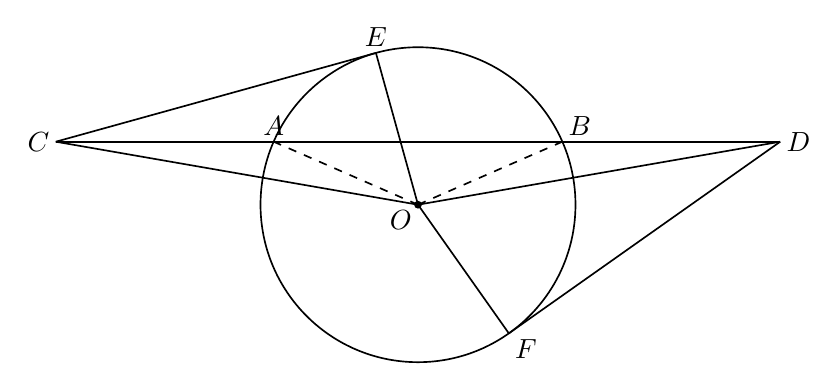
\begin{tikzpicture}[x=1cm,y=1cm,line width=.6pt,font=\normalsize]
\coordinate (O) at (0.0000,0.0000);
\coordinate (A) at (-1.8330,0.8000);
\coordinate (B) at (1.8330,0.8000);
\coordinate (C) at (-4.6000,0.8000);
\coordinate (D) at (4.6000,0.8000);
\coordinate (E) at (-0.5344,1.9273);
\coordinate (F) at (1.1537,-1.6337);
\draw (O) circle[radius=2.0000];
\draw (C)--(D);
\draw (C)--(E);
\draw (C)--(O);
\draw (O)--(D);
\draw (O)--(E);
\draw (O)--(F);
\draw (D)--(F);
\draw[dashed] (O)--(A);
\draw[dashed] (O)--(B);
\node[left=2pt,inner sep=0pt] at (C) {$C$};
\node[above=2pt,inner sep=0pt] at (A) {$A$};
\node[above right=2pt,inner sep=0pt] at (B) {$B$};
\node[right=2pt,inner sep=0pt] at (D) {$D$};
\node[above=2pt,inner sep=0pt] at (E) {$E$};
\node[below right=2pt,inner sep=0pt] at (F) {$F$};
\node[below left=2pt,inner sep=0pt] at (O) {$O$};

% Explicit named circle-center points, painted after all region fills.
\fill (O) circle[radius=1.4pt];
\end{tikzpicture}
